\documentclass[../main.tex]{subfiles}

\begin{document} %%%%%%%%%%%%%%%%%%%%%%%%%%%%%%%%%%%%%%%%%%%%%%%%%%%%%%%%%%%%
\section{Grafos} 
    Lista de reproducción YouTube \cite{grafos_lista_youtube}.

    \subsection{Propiedades}
    
    % Cargamos la imagen
    \begin{figure}[ht]
        \centering
        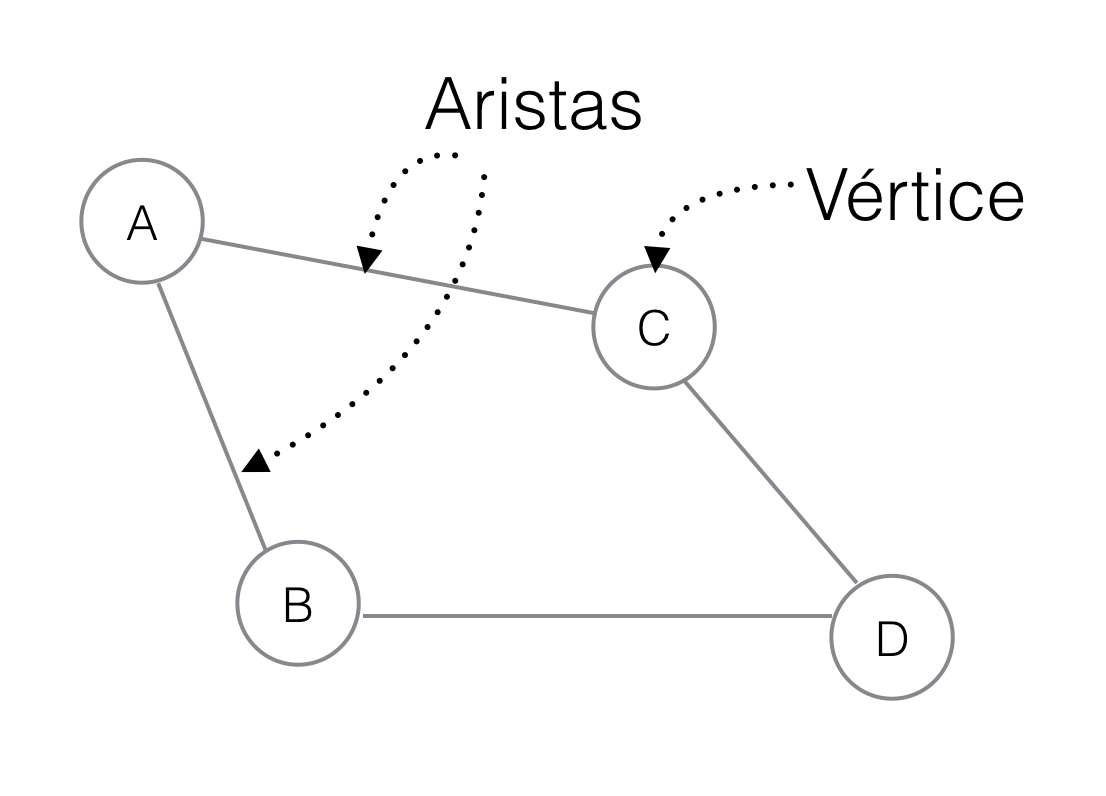
\includegraphics[width=0.5\textwidth]{images/grafos/grafo_aristas_vertices.png}
        \caption{Grafos Aristas = Edge y Vértices o Nodos = Vertex }
    \end{figure}


    \begin{enumerate}
        \item \textbf{Grafos orientados} (o dirigidos o digrafos) si las aristas (o arcos) que conectan sus vertices
        (también llamados nodos) están orientadas.
        \item \textbf{Grafos no orientados} (o no dirigidos) si las aristas que conectan sus vertices no están
        orientadas.
            % Cargamos la imagen
            \begin{figure}[ht]
                \centering
                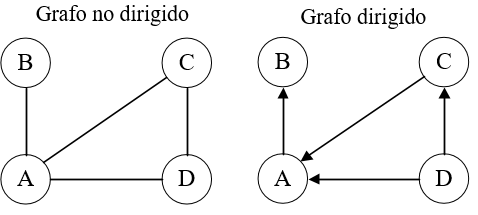
\includegraphics[width=0.5\textwidth]{images/grafos/grafos_dirigido.png}
                \caption{Grafos Dirigido y No Dirigido}      
            \end{figure}

        \item \textbf{Ciclo:} camino que conteniendo vertices distintos, excepto el primero que coincide con el ultimo.
            % Cargamos la imagen
            \begin{figure}[ht]
                \centering
                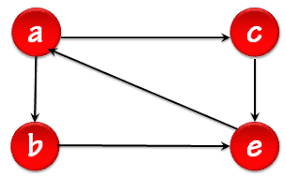
\includegraphics[width=0.3\textwidth]{images/grafos/grafo_ciclo.png}
                \caption{Grafos Ciclo: $a \rightarrow b \rightarrow e \rightarrow a$, longitud 3.}
                \label{fig:grafos_ciclo}     
            \end{figure}

        \item \textbf{Grafo no dirigido conexo:} Grafo no orientado es conexo si para todo vértice del grafo hay un camino que lo conecte con otro vertice cualquiera del grafo.
            % Cargamos la imagen
            \begin{figure}[ht]
                \centering
                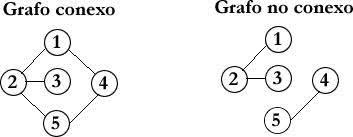
\includegraphics[width=0.5\textwidth]{images/grafos/grafo_conexo.jpeg}
                \caption{Grafos Conexo y No Conexo}
            \end{figure}
        
        \item \textbf{Grafo dirigido fuertemente conexo:} Grafo dirigido es fuertemente conexo sii entre cualquier par de vértices hay un camino que los une. Ver Figura \ref{fig:grafos_ciclo}.
        
        \item \textbf{Árbol libre:} Grafo no dirigido conexo sin ciclos.
            % Cargamos la imagen
            \begin{figure}[ht]
                \centering
                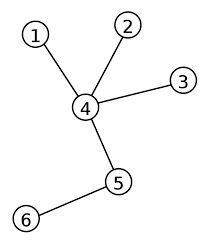
\includegraphics[width=0.3\textwidth]{images/grafos/grafo_arbol_libre.png}
                \caption{Grafos Árbol Libre}
            \end{figure}
    \end{enumerate}
    
    \newpage

    \subsection{Estructuras para implementar grafos}

        \subsubsection{Matriz de Adyacencia}
            % Cargamos la imagen
            \begin{figure}[ht]
                \centering
                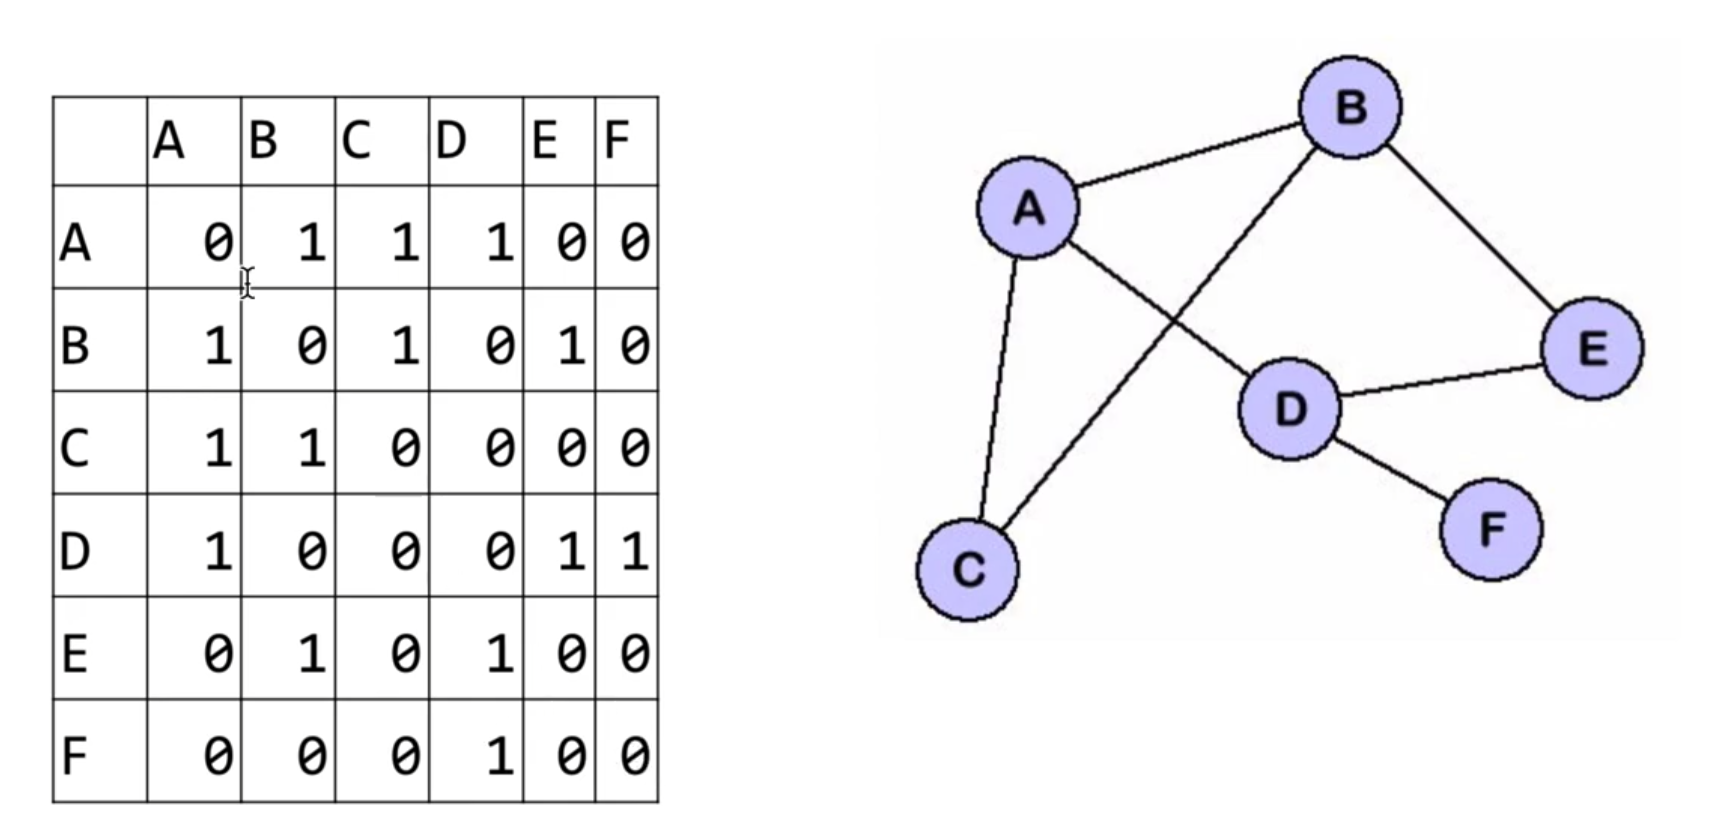
\includegraphics[width=0.8\textwidth]{images/grafos/grafo_matriz_adyacencia_1.png}
                \caption{Grafo no dirigido y no pesado Matriz de Adyacencia} 
            \end{figure}

            % Cargamos la imagen
            \begin{figure}[ht]
                \centering
                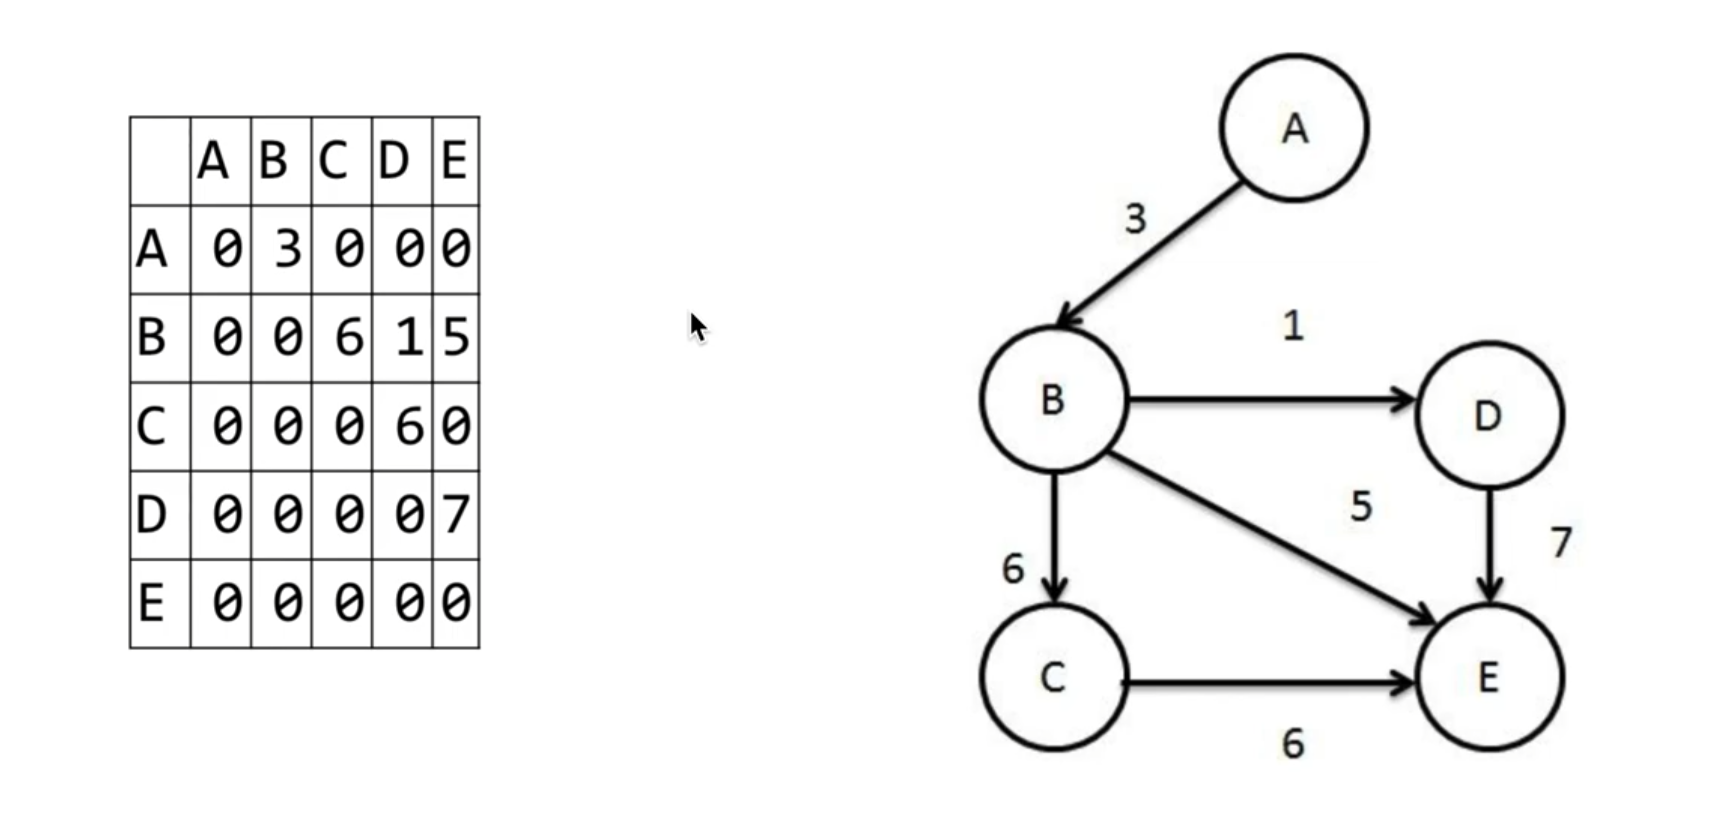
\includegraphics[width=0.8\textwidth]{images/grafos/grafo_matriz_adyacencia_2}
                \caption{Grafo dirigido y pesado Matriz de Adyacencia} 
            \end{figure}
            
            \newpage

        \subsubsection{Matriz de Incidencia}
            % Cargamos la imagen
            \begin{figure}[ht]
                \centering
                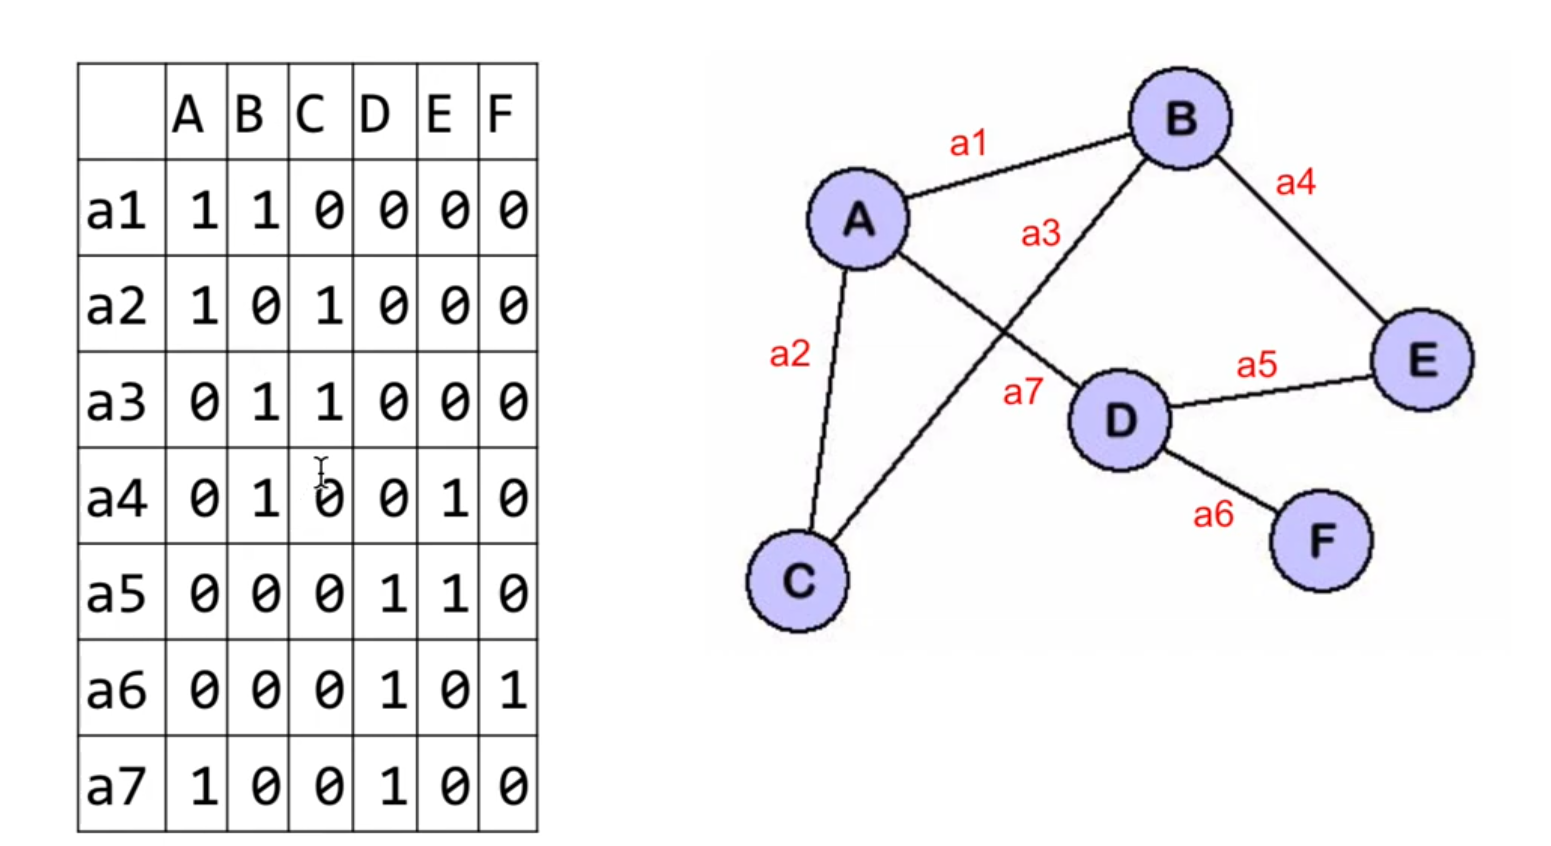
\includegraphics[width=0.8\textwidth]{images/grafos/grafo_matriz_incidencia_1.png}
                \caption{Grafo no dirigido y no pesado Matriz de Incidencia} 
            \end{figure}

            % Cargamos la imagen
            \begin{figure}[ht]
                \centering
                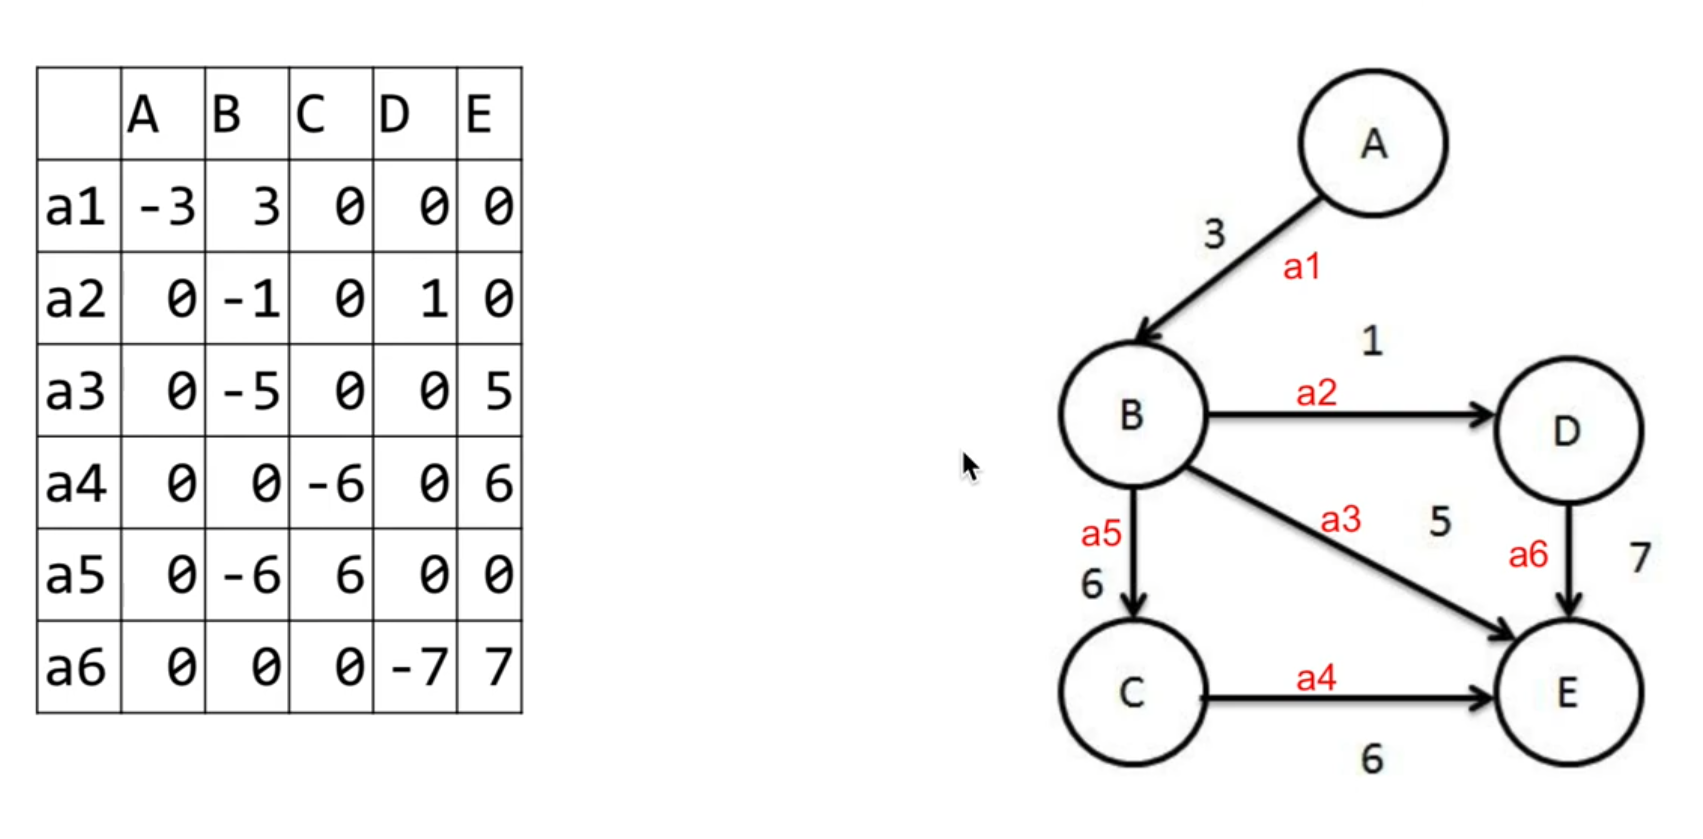
\includegraphics[width=0.8\textwidth]{images/grafos/grafo_matriz_incidencia_2.png}
                \caption{Grafo dirigido y pesado Matriz de Incidencia} 
            \end{figure}

            \newpage

            \subsubsection{Complejidad}
    
                \begin{table}[ht]
                    \centering
                    \begin{tabular}{|l|l|l|l|}
                    \hline
                        & M. Incidencia & M. Adyacencia & Lista Adyacencia\\ \hline
                        \textbf{Espacio:} & $O(V \cdot E)$ & $O(V^2)$ & $O(V + E)$\\ \hline
                        \textbf{Agregar un vértice:}  & $O(V \cdot E)$ & $O(V^2)$ & $O(1)$ o $O(V)$\\ \hline
                        \textbf{Agregar una arista:} & $O(V \cdot E)$ & $O(1)$ & $O(V)$ \\ \hline
                        \textbf{Si dos vértices son adyacentes:} & $O(E)$ & $O(1)$ & $O(V)$\\ \hline
                        \textbf{Obtener los abyacentes de un vértices:} & $O(E)$ & $O(V)$ & $O(V)$\\ \hline
                    \end{tabular}
                    \caption[short]{Coplejidad.}
                \end{table}

        \subsection{Recorridos Grafos}
            \underline{Recorridos Grafos Dirigidos}
            \begin{itemize}
                \item Anchura: BFS (Breadth First Search)
                \item Profundidad: DFS (Depth First Search)
            \end{itemize}

            Ver Videos YouTube \cite{grafo_bfs_dfs_youtube_1} y \cite{grafo_bfs_dfs_youtube_2}.

            \subsubsection{BFS: Recorrido en Anchura}
                Para grafos dirigidos y no dirigidos.\\
                
                \underline{Procedimento:}
                \begin{itemize}
                    \item Seleccionar un vértice inicial.
                    \item Marcarlo como visitado.
                    \item Encolarlo.
                    \item Mientras la \textbf{cola} (FIFO) no esté vacía :
                        \begin{itemize}
                            \item Desencolar vértice.
                            \item Mostrarlo.
                            \item Marcar como visitados.
                                \begin{itemize}
                                    \item Los vertices adyacentes no visitado.
                                \end{itemize}
                                \item Encolarlos.
                        \end{itemize}

                \end{itemize}

            \subsubsection{DFS: Recorrido en Profundidad}
                Para grafos dirigidos y no dirigidos.\\
                
                \underline{Procedimento:}
                \begin{itemize}
                    \item Seleccionar un vértice inicial.
                    \item Marcarlo como visitado.
                    \item Apilarlo.
                    \item Mientras la \textbf{pila} (LIFO) no esté vacía :
                        \begin{itemize}
                            \item Desapilar vértice.
                            \item Mostrarlo.
                            \item Recorrer todos los vértices adyacentes del vértice desapilado
                                \begin{itemize}
                                    \item Si el vértice adyacente no ha sido visitado, marcarlo como visitado y apilarlo.
                                    \item Si el vértice adyacente ya ha sido visitado, continúa con el siguiente vértice adyacente.
                                \end{itemize}
                        \end{itemize}
                \end{itemize}

            \subsubsection{Complejidad BFS y DFS}
                
                \begin{table}[ht]
                    \centering
                    \begin{tabular}{|l|l|l|}
                    \hline
                    & Matriz Adyacencia & Matriz Incidencia  \\ \hline
                    Anchura BFS & $O(V^2)$ & $O(V+E)$ \\ \hline
                    Profundidad DFS & $O(V^2)$ & $O(V+E)$  \\ \hline
                    \end{tabular}
                    \caption[short]{Coplejidad.}
                \end{table}

            \subsubsection{Aplicaciones}
                \underline{DFS: Recorrido Profundidad}
                \begin{enumerate}
                    \item \textbf{Test de Aciclidad (Ciclos):} Si al recorrer un grafo con DFS se encuentra un vértice que ya fue visitado, entonces existe un ciclo.
                    \item  \textbf{Puntos de Articulación:} Un punto de articulación es un vértice que al ser eliminado aumenta la cantidad de componentes conexas del grafo.
                    \item \textbf{Obtención de las componentes fuertemente conexas en un grafo dirigido:} Una componente fuertemente conexa es un subgrafo en el que para cada par de vértices existe un camino de uno a otro.
                \end{enumerate}

                \underline{BFS: Recorrido Anchura}
                \begin{enumerate}
                    \item \textbf{Camino mínimo:} Si el grafo es no pesado, el camino mínimo entre dos vértices es el camino que tiene menos aristas.
                    \item \textbf{Árbol de expansión mínimo:} Si el grafo es pesado, el árbol de expansión mínimo es el subgrafo que tiene todos los vértices del grafo original y la suma de los pesos de sus aristas es la mínima posible.
                \end{enumerate}


\end{document}  %%%%%%%%%%%%%%%%%%%%%%%%%%%%%%%%%%%%%%%%%%%%%%%%%%%%%%%%%%%%%